\subsection{Реализация процессов}

Разработанное программное средство включает набор взаимосвязанных процессов, обеспечивающих полный цикл работы системы обнаружения аномалий: от взаимодействия с пользователем и источником данных до обучения модели и выполнения детектирования. Общая схема основных процессов программного средства представлена на рисунке~\ref{fig:processes_overview}.

\begin{figure}
    \centering
    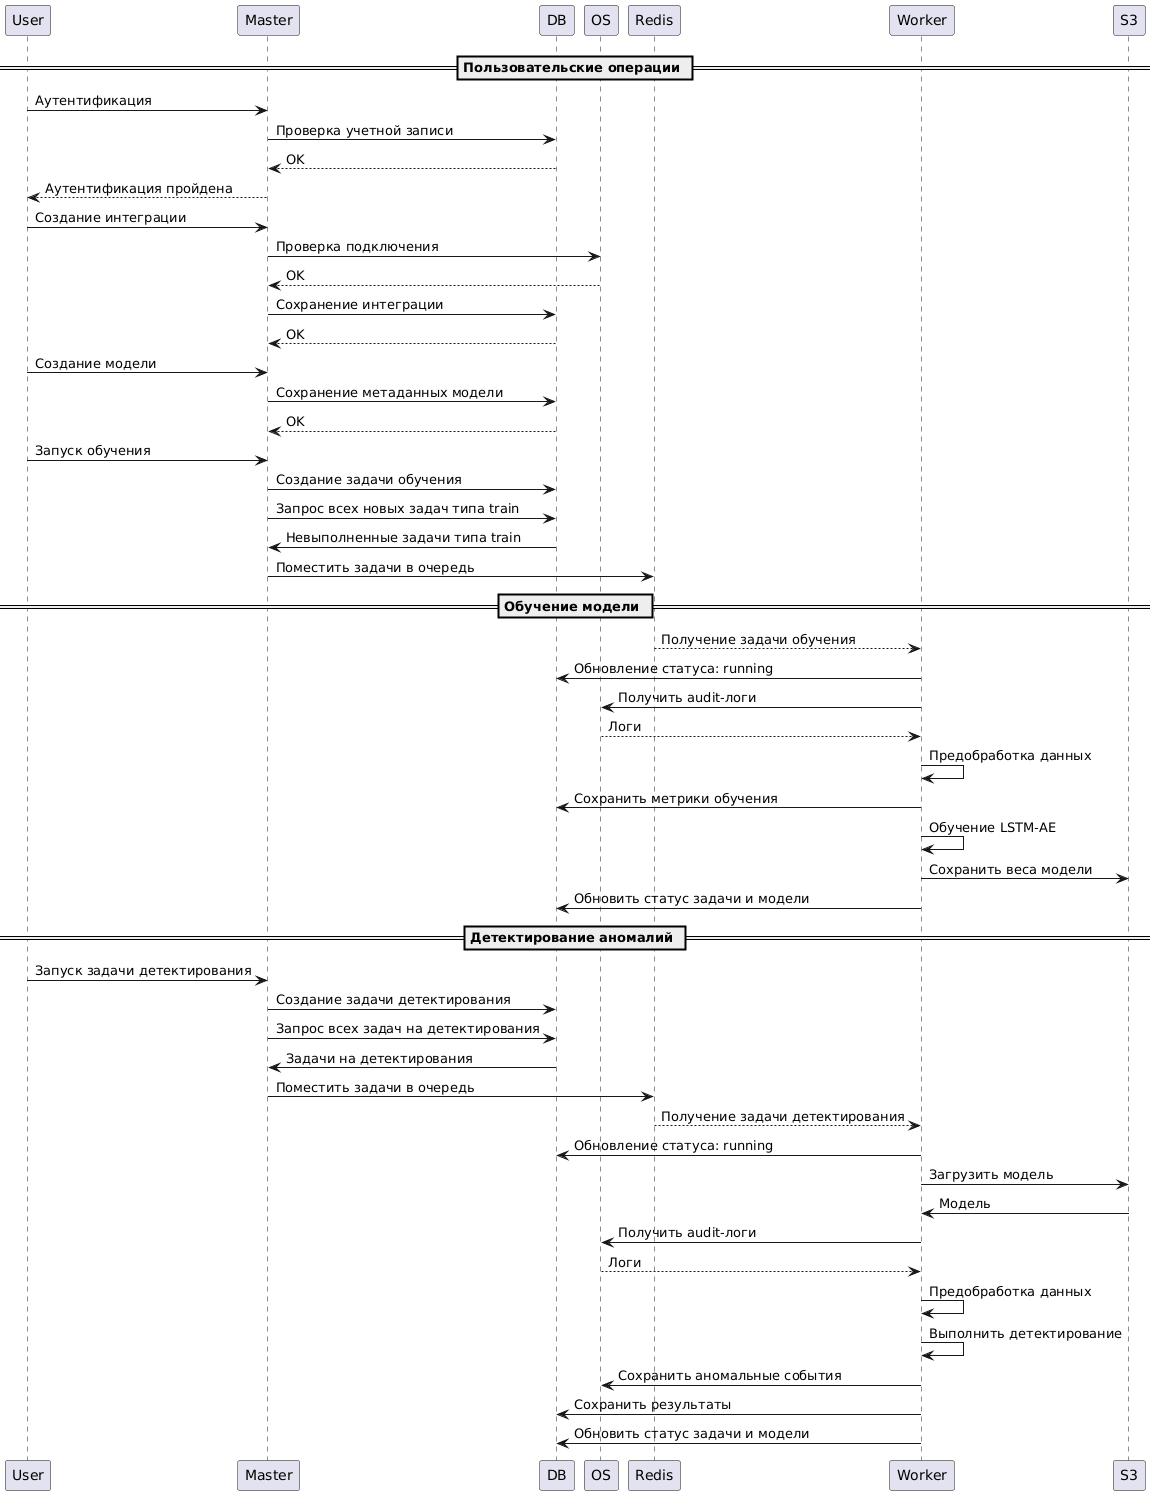
\includegraphics[scale=0.36]{inc/images/processes_overview}
    \caption{Общая схема процессов программного средства}
    \label{fig:processes_overview}
\end{figure}

Основные процессы системы можно разделить на две группы. К первой группе относятся процессы, связанные с управлением пользователями и настройкой системы: регистрация, аутентификация, создание интеграции с OpenSearch и создание модели обнаружения аномалий. Данные процессы выполняются через центральный компонент системы и не требуют запуска ресурсоёмких вычислений. Их результатом является формирование записей в базе данных и подготовка параметров для последующего создания задач на обучение или детектирование аномалий.

Ко второй группе относятся процессы, связанные с обработкой данных и работой НС. К ним относятся запуск обучения модели, запуск режима обнаружения аномалий, получение данных из OpenSearch, формирование признакового описания и вычисление итоговых метрик. Данные операции выполняются асинхронно с использованием worker-компонентов и очереди задач Redis, что позволяет не блокировать основной поток обработки пользовательских запросов.

Процесс аутентификации начинается с обращения пользователя к компоненту Master, который выполняет проверку учётной записи в базе данных PostgreSQL. После успешной проверки система возвращает результат аутентификации пользователю. Аутентификация реализуется на основе проверки логина и пароля с последующим формированием токена доступа, который используется для обращения к защищённым методам API.

Процесс создания интеграции с OpenSearch включает указание параметров подключения, таких как адрес сервера, имя пользователя, пароль и имя индекса. После сохранения параметров выполняется проверка корректности подключения к источнику данных. В случае успешной проверки информация об интеграции сохраняется в базе данных и становится доступной для последующего использования при обучении модели и детектировании аномалий.

Аналогичным образом при создании модели Master формирует и сохраняет метаданные модели, соответствующие этапу её жизненного цикла.

\subsection{Обучение модели НС}

Процесс обучения модели является одним из ключевых в разработанном программном средстве. Инициация обучения осуществляется пользователем через API центрального компонента системы. При этом создаётся задача типа \textit{train} со статусом \textit{starting}, информация о которой сохраняется в базе данных. Функции планирования выполнения задач реализованы в составе компонента Master. Планировщик периодически выполняет опрос базы данных с целью получения новых задач обучения, не отправленных ранее в очередь. Для таких задач статус изменяется на \textit{pending}, после чего они помещаются в очередь сообщений Redis для последующей асинхронной обработки.

Worker-компонент извлекает задачу из очереди, переводит её в состояние \textit{running} и приступает к выполнению. На первом этапе осуществляется загрузка audit-логов из OpenSearch. Полученные данные проходят процедуру предобработки, включающую очистку, нормализацию и формирование последовательностей признаков фиксированной длины. На следующем этапе выполняется обучение модели на основе архитектуры LSTM-AE с использованием подготовленных данных. В процессе обучения вычисляются метрики, характеризующие эффективность модели, которые сохраняются в БД. По завершении обучения веса модели сохраняются во внешнем хранилище.

После успешного завершения всех этапов модель переводится в состояние \textit{ready}, что делает её доступной для использования в задачах обнаружения аномалий. Статус соответствующей задачи обновляется на \textit{done}, что свидетельствует о завершении процесса обучения.

Блок-схема алгоритма обучения приведена на рисунке~\ref{fig:train_process}.

\begin{figure}
    \centering
    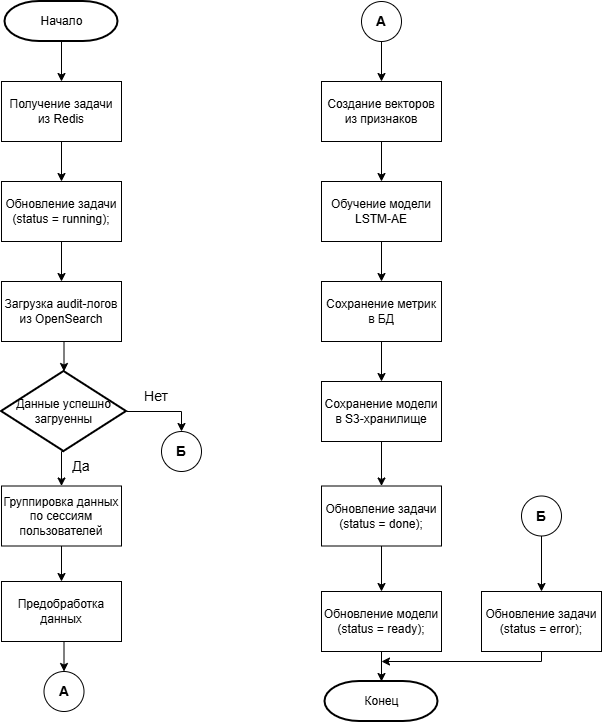
\includegraphics[scale=0.4]{inc/images/train_process}
    \caption{Блок-схема алгоритма обучения}
    \label{fig:train_process}
\end{figure}

\subsection{Обнаружение аномалий}

Процесс обнаружения аномалий реализуется по аналогичному принципу. Пользователь инициирует выполнение задачи типа \textit{detect} со статусом \textit{starting}, информация о которой сохраняется в базе данных. Планировщик периодически выполняет запрос к базе данных для получения новых задач обнаружения аномалий со статусом \textit{starting}, которые ранее не были отправлены в очередь. Для таких задач статус изменяется на \textit{pending}, после чего они помещаются в очередь сообщений Redis для последующей обработки.

Worker-компонент извлекает задачу из очереди и переводит её в состояние \textit{running}. На первом этапе осуществляется получение актуальных audit-логов из OpenSearch. Далее данные преобразуются в формат, совместимый с входом обученной модели, включая предобработку и формирование последовательностей признаков.

После подготовки данных выполняется вычисление показателя аномальности с использованием обученной модели LSTM-AE. В случае, если значение ошибки превышает заданный порог, соответствующее событие классифицируется как аномальное. Все аномальные события сохраняются в отдельном индексе OpenSearch

Результаты анализа сохраняются в базе данных и используются для последующего отображения пользователю. После завершения обработки задача переводится в состояние \textit{starting}, чтобы планировщих смог ее запланировать в очереди.

Блок-схема алгоритма обнаружения аномалий приведена на рисунке~\ref{fig:detect_process}.

\begin{figure}
    \centering
    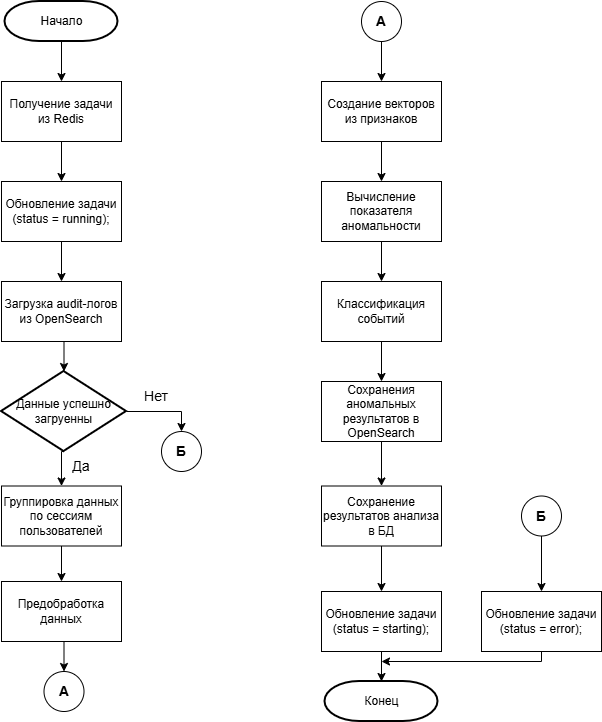
\includegraphics[scale=0.4]{inc/images/detect_process}
    \caption{Блок-схема алгоритма обнаружения аномалий}
    \label{fig:detect_process}
\end{figure}
